% LaTeX template for MSc. and BSc. theses at the Department of Hydraulic Engineering and Water Resources Management (University of Stuttgart)
% Latest release: v3.0.0 (June 2024)
% Original Author: Beatriz Negreiros
% Contributors: Sebastian Schwindt
% Change log:
%	v3.0.0: - replaced style file with a class file

% DISCLAIMER
% While this template complies with basic style requirements, it is the thesis author's responsibility to assure that all requirements are in complieance with the school, department/institute and/or degree program.

\documentclass[11pt,twoside]{thesis}	

% Document
\title{\textbf{Thesis Title}} % enter the titlename of your thesis here
\author{Student Name} % enter your name

% Macros - here you can define macros for shortening the writing of large words, for instance:
\def\rmse{Root Mean Squared Error}
\def\std{Standard Deviation}



% BEGINNING OF THE DOCUMENT
\begin{document}

\begin{titlepage}
	\begin{center}
	
\includegraphics[width=6cm]{uni_logo_1.png}\hspace*{6cm} % horizontal space
	
\includegraphics[width=3cm]{Logo_LWW.png}\\

		\vspace{3cm} % vertical space
		
		\large [Name of the department]\\
		
		\large [Name of the institute]\\
		
		\vspace{3cm} % vertical space

		\Huge\textbf{[Thesis name]}\\

		\vspace{1.5cm} % vertical space
		
		\Large Master's Thesis % It's not Master Thesis, nor master thesis, but exactly how it's written here
		
		\vspace{1.5cm} % vertical space
		
		\large Student's name\\
		\large (Course's name)
		
		\vspace{2cm} % vertical space
		
		\large [Matriculation Number] \\
		
		\Large \date{\today}
	\end{center}
		\vspace{1.5cm} % vertical space
		\begin{tabular}{rl}
			\textbf{Examiner:} & [Name of examiner] \\
			\textbf{Supervisors:} & [Supervisor 1] \\ & [Supervisor 2]
		\end{tabular}
	
\end{titlepage}
		

\newpage\null\thispagestyle{empty}\newpage

\pagenumbering{roman}

\chapter*{Declaration}
{
	I declare that I have developed and written the enclosed thesis completely by myself and that I have not used sources or means without declaration in the text. Any thoughts from others or literal quotations are clearly marked. The thesis was not used in the same or in a similar version to achieve an academic grading or is being published elsewhere. The enclosed electronic version is identical to the printed versions.\\
	
	% Comment out the following paragraph only if you have not used a large language model (LLM) such as ChatGPT
	The main text, ideas, analyses, and conclusions presented in this thesis are my own, produced without the use of artificial intelligence (AI) tools for creative or substantive writing. I confirm that AI language models (e.g., ChatGPT) were only used to provide assistance in spelling, grammar, and minor editorial refinements. These tools were not employed in generating new content, forming arguments, or conducting the research work described. I take full responsibility for the originality, accuracy, and integrity of the thesis.\\ 
	
	I agree that the present work is made available for scientific purposes in the libraries of the Institute for Water and Environmental Systems, University of Stuttgart (published according § 6 Abs. 1 UrhG (Copyright Act) and thereof can be cited under § 51 of the UrhG (Copyright Act).
}

\chapter*{Acknowledgments}
{
add your Acknowledgments
}

\chapter*{Abstract}
{
Abstracts should not be more than one page. A thesis written in Germany requires an additional English abstract. 
}

% List of contents, figures and tables
\tableofcontents
\clearpage

\listoffigures
\addcontentsline{toc}{chapter}{List of Figures}

\listoftables
\addcontentsline{toc}{chapter}{List of Tables}

\addcontentsline{toc}{chapter}{Notation}
\chapter*{Notation}
\markboth{Notation}{Notation}
\section*{Roman letters}
\begin{longtable}{l  @{\hspace{1em}} l @{\hspace{1em}} L{0.73\textwidth}}
\textbf{Letter} & \textbf{Unit} & \textbf{Description} \\
\multicolumn{3}{p{\textwidth}}{}\\ % Force table to expand to textwidth and flush left
$x$& m & streamwise coordinate, pointing in the upstream direction\\
$y$& m & spanwise coordinate, pointing toward the right bank\\
$z$& m & vertical coordinate, pointing against gravity acceleration vector \\
\end{longtable}
\addtocounter{table}{-1}

\section*{Greek letters}
\begin{longtable}{l  @{\hspace{1em}} l @{\hspace{1em}} L{0.8\textwidth}}
\textbf{Letter} & \textbf{Unit} & \textbf{Description} \\
\multicolumn{3}{p{\textwidth}}{}\\ % Force table to expand to textwidth and flush left
$\eta$ & -- & porosity \\
$\Phi$ & -- & dimensionless bedload transport\\
\end{longtable}
\addtocounter{table}{-1}

\section*{Acronyms, abbreviations, and subscripts}
\begin{longtable}{l  @{\hspace{1em}} l}
\multicolumn{2}{p{\textwidth}}{}\\
CFD & Computational Fluid Dynamics\\
GIS & Geographic Information System\\
GUI & Graphical User Interface\\
OS & Operating System\\

\end{longtable}
\addtocounter{table}{-1}

\textit{Note: SI unit abbreviations like "a" for \textit{annum} or "m" for \textit{meter} are not listed.}


% Beginning of chapters
\pagestyle{fancy}
\fancyhf{}
\fancyhead[LE,RO]{\nouppercase{\leftmark}}
\fancyhead[RE,LO]{\nouppercase{\rightmark}}
\fancyfoot[LE,RO]{\thepage}
\renewcommand{\headrulewidth}{1.0pt}

\chapter{Introduction}
% \chapter{Einleitung}
\label{ch:introduction}

\pagenumbering{arabic}
\setcounter{page}{1}



\section{Background}
\label{subsec:background}
write here

\section{Something Location}
\label{subsec:somelocation}

write here

See more in ~\autoref{subsec:background}
write here
	
\begin{center}
\end{center}
\cleardoublepage

\chapter{State-of-the-Art}
%\chapter{Theoretische Grundlagen}
\label{ch:soa}

% This chapter can be also called Literature Review

Check what others have done, which is relevant to your research question and to provide evidence for testing the hypotheses defined in \autoref{sec:rq}.

For coherence: note that chapter titles should be \textit{Camel Cased}, while everything else is \textit{Sentence cased}, including all kinds of section names.

\section{Previous works}
\label{sec:prevworks}
	
% For referring to sections or chapter you rpesented before:
As explained in \citeA{negreiros2024database}.
	
	
\section{Types of something and image manipulation}
\label{sec:typesome}

Do \citeA{kundu2008fluid} talk about Lagrangian and Eulerian concepts visualized in \autoref{fig:example}?

Note that saving graphics in JPG format is usually the best option, and PNG is only useful for charts with low pixel coverage.

JPG is uitable for photographs and complex images where a smaller file size is important. It uses lossy compression, which reduces file size substantially. When using the JPG format for a thesis report, be sure to save at 300 dpi (dots per inch).

PNG is best used when you need lossless compression (heavy files!) and transparency support. It is ideal for charts with sharp edges, text, or areas of \textbf{solid} color, as it preserves detail without introducing compression artifacts.

GNU Image Manipulation Program, GIMP, is a powerful open-source image editing software suitable for a wide range of tasks, including photo retouching, image composition, and graphic design. It supports various file formats, including PNG and JPG, and provides advanced tools such as layer management, customizable brushes, and color correction features. GIMP is an excellent free alternative to commercial software, making it a great choice for students who ambition high-quality image editing capabilities without licensing costs.


\begin{figure}[htp]
	\begin{center}
		\begin{minipage}{\textwidth}
			\centering
			\resizebox*{.9\textwidth}{!}{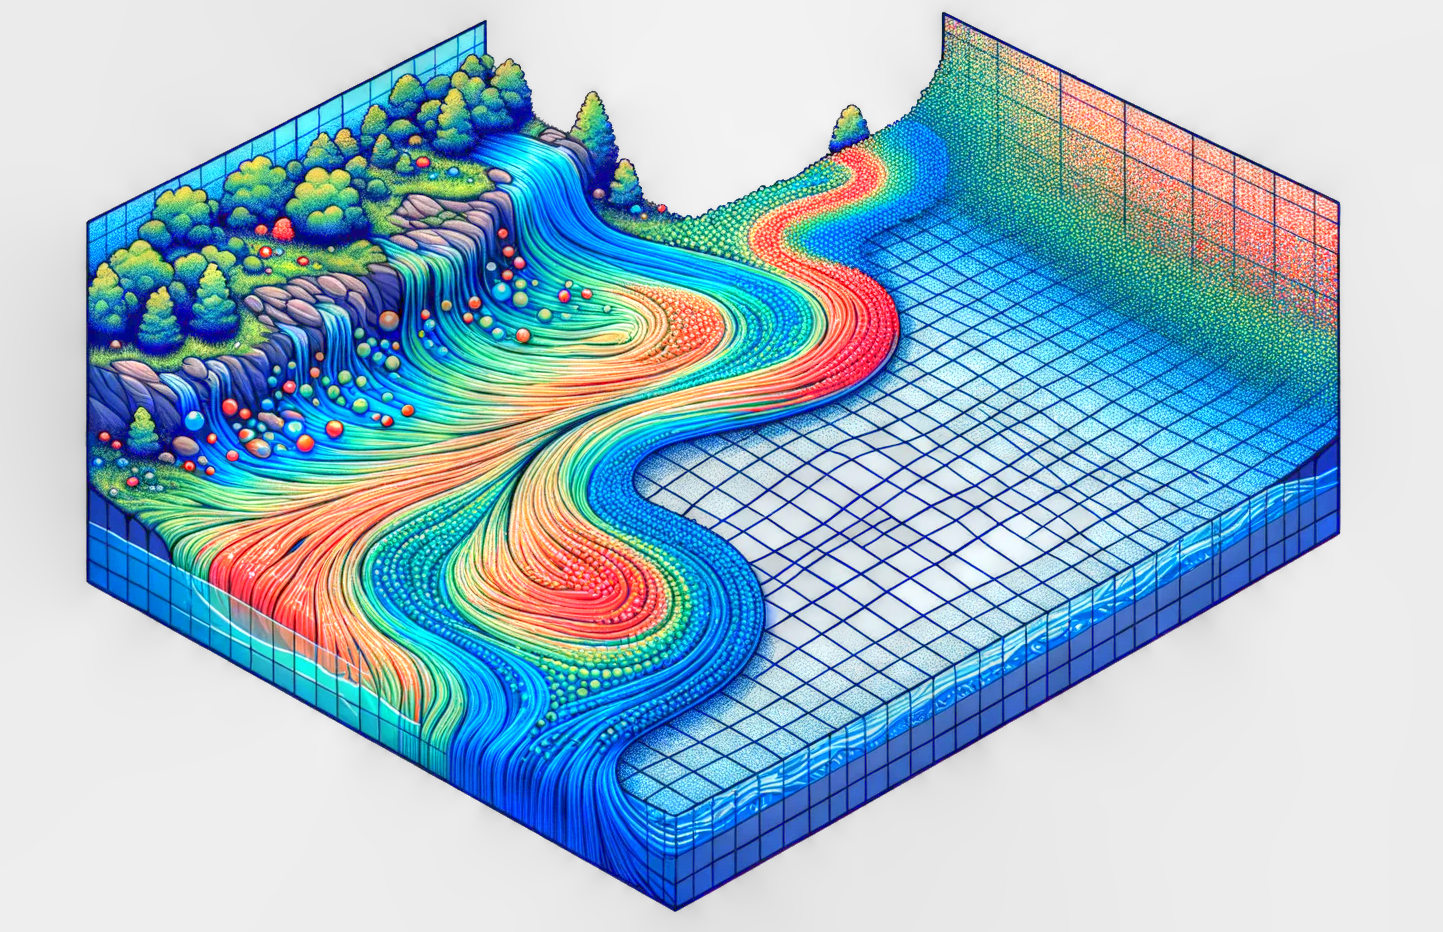
\includegraphics{example}}
			\caption[An example figure.]{An example figure that visually tries to integrate Lagrangian and Eulerian concepts.}
			\label{fig:example}
		\end{minipage}
	\end{center}
\end{figure}

		
\subsection{A subsection with table}
\label{subsec:somesome}
		
As the \autoref{tab:typesomething} shows, this text has to introduce the thing before the table lists the use of the thing.
		
		
\begin{table}[hb] % try [h]ere, then [b]ottom to make sure the table is mentioned in the text before it is shown
	\centering
	\caption{Captions of tables should be positioned above the table, while figure captions should be in the bottom}
	\begin{tabular}{ll}
		\hline
		\textbf{Thing} & \textbf{Use} \\
		\hline
		something & something \\
		something & something \\
		something & something \\
		\hline
	\end{tabular}
	% the label goes below the tabular env
	\label{tab:typesomething}
\end{table}
		
\subsection{No subsection goes alone}
\label{subsec:somenoth}

And it should also have some text.


\section{Something statistics with an equation}
\label{sec:somestatistics}
	
As shown in \autoref{eq:happiness}
\begin{equation}\label{eq:happiness}
	\mbox{happiness}=\frac{\mbox{EmptyCup}+\mbox{FavoriteDrink}}{\mbox{EmptyCups}}
\end{equation}	
	
\section{A section header}
\label{sec:some-ref}
	
\subsection{The logic underlying something in a DEF BOX}
\label{subsec:logicunderlying}
    	
\defbox{The thing}{
	This is the definition of the thing.
}
    	
\subsection{Concepts and terminology}
\label{subsec:conceptsterm}	
		
\subsubsection*{Something set rules} 

Understanding the semantics of something

\section{Something or nothing?}
\label{sec:someornot}

\subsubsection*{Unnumbered non-sense header?}

\infobox{The note}{
	Do you really need to do so much numbering?
}
   	
    	
    


\chapter{Methods} % NOT: Methodology
% \chapter{Laboruntersuchungen}
% \chapter{Methoden}
\label{ch:methods}

Describe the methods that \textbf{you} use to answer the research question. Remember: your goal is to provide a pathway for testing the hypotheses defined in \autoref{sec:rq}.

\section{Algorithms}

To explain your algorithms, use the boilerplate templates from our thesis class. For example:

\begin{lstlisting}
def add_one(par):
	"""
	:param int par: an integer input parameter
	
	A simple function that adds one
	"""
	return par += 1
\end{lstlisting}

Single commands or \inlinecode{function_names} can be written using the \inlinecode{\inlinecode} for general code, \inlinecommand{python run_script.py} for shell commands, or \inlinecode{\inlinepy} for \inlinepy{python_items}.

\section{Commands}

Commands send to terminal can be written in a terminal environment, for instance, with guidance for cloning a repository:

\begin{terminal}
	 git clone https://github.com/Ecohydraulics/latex-thesis-template
\end{terminal}

In-line, commands like \inlinecode{git clone} can be added.

However, for directories and filenames, use \texttt{/dir/to/code.py}.
	

\chapter{Results}
% \chapter{Ergebnisse}
\label{ch:results}

\chapter{Discussion}
%\chapter{Diskussion}
\label{ch:discussion}

Describe logical links that can be inferred from your results here. How do the results help to test the hypotheses stated in \autoref{sec:rq}?

\begin{itemize}
	\item Do not write: "The hypothesis is True" or "The hypothesis is False".
	\item Do write: "No evidence was found that the hypothesis is false." or "Evidence was found that the hypothesis is false."
\end{itemize}


\infobox{Why so complicated?}{
	From a scientific perspective, we can never be absolutely sure about the truth of a hypothesis. This is why we need to use this complicated writing.
}

Now, how does this help answering the research question?



\chapter{Conclusions}
%\chapter{Fazit}
\label{ch:conclusion}

Not an abstract: summary of NEW INSIGHTS GAINED FROM THIS THESIS BASED ON THE RESEARCH QUESTION, and as per the discussion.



\pagestyle{fancy}
\fancyhf{}
\fancyhead[LE,RO]{\nouppercase{\rightmark}}
\fancyfoot[LE,RO]{\thepage}
\renewcommand{\headrulewidth}{1.0pt}

\bibliographystyle{apacite}
\bibliography{hydro-informatics}


% The \appendix statement indicates the beginning of the appendices.
\appendix
% Add an un-numbered title page before the appendices and a line in the Table of Contents
\chapter*{Appendices}
\addcontentsline{toc}{chapter}{Appendices}
% Appendices are just more chapters, with different labeling (letters instead of numbers).
\chapter[Appendix]{Something to Complement}
\label{AppendixA}
% Tip 4: Example (above) of how to get a shorter chapter title for the Table of Contents 
%======================================================================

\section{[Maps of Something]}


\end{document}
